\documentclass[11pt,fleqn, oneside,openany]{book} % Default font size and left-justified equations

% use this list: https://www.educative.io/blog/google-coding-interview

%%%%%%%%%%%%%%%%%%%%%%%%%%%%%%%%%%%%%%%%%%%%
%               Structure
%%%%%%%%%%%%%%%%%%%%%%%%%%%%%%%%%%%%%%%%%%%%
%%%%%%%%%%%%%%%%%%%%%%%%%%%%%%%%%%%%%%%%%
% The Legrand Orange Book
% Structural Definitions File
% Version 2.0 (9/2/15)
%
% Original author:
% Mathias Legrand (legrand.mathias@gmail.com) with modifications by:
% Vel (vel@latextemplates.com)
% 
% This file has been downloaded from:
% http://www.LaTeXTemplates.com
%
% License:
% CC BY-NC-SA 3.0 (http://creativecommons.org/licenses/by-nc-sa/3.0/)
%
%%%%%%%%%%%%%%%%%%%%%%%%%%%%%%%%%%%%%%%%%

%----------------------------------------------------------------------------------------
%	VARIOUS REQUIRED PACKAGES AND CONFIGURATIONS
%----------------------------------------------------------------------------------------

\usepackage[top=3cm,bottom=3cm,left=3cm,right=3cm,headsep=10pt,a4paper]{geometry} % Page margins

\usepackage{graphicx} % Required for including pictures
\graphicspath{{images/}} % Specifies the directory where pictures are stored

\usepackage{lipsum} % Inserts dummy text

\usepackage{tikz} % Required for drawing custom shapes

\usepackage[english]{babel} % English language/hyphenation

\usepackage{enumitem} % Customize lists
\setlist{nolistsep} % Reduce spacing between bullet points and numbered lists

\usepackage{booktabs} % Required for nicer horizontal rules in tables

\usepackage{xcolor} % Required for specifying colors by name
\definecolor{ocre}{RGB}{243,102,25} % Define the orange color used for highlighting throughout the book

%----------------------------------------------------------------------------------------
%	FONTS
%----------------------------------------------------------------------------------------

\usepackage{avant} % Use the Avantgarde font for headings
%\usepackage{times} % Use the Times font for headings
\usepackage{mathptmx} % Use the Adobe Times Roman as the default text font together with math symbols from the Sym­bol, Chancery and Com­puter Modern fonts

\usepackage{microtype} % Slightly tweak font spacing for aesthetics
\usepackage[utf8]{inputenc} % Required for including letters with accents
\usepackage[T1]{fontenc} % Use 8-bit encoding that has 256 glyphs

%----------------------------------------------------------------------------------------
%	BIBLIOGRAPHY AND INDEX
%----------------------------------------------------------------------------------------

\usepackage[citestyle=numeric,sorting=nyt,sortcites=true,autopunct=true,babel=hyphen,hyperref=true,abbreviate=false,backref=true,backend=biber]{biblatex}
\addbibresource{sources/bibliography.bib}
\defbibheading{bibempty}{}

\usepackage{calc} % For simpler calculation - used for spacing the index letter headings correctly
\usepackage{makeidx} % Required to make an index
\makeindex % Tells LaTeX to create the files required for indexing

%----------------------------------------------------------------------------------------
%	MAIN TABLE OF CONTENTS
%----------------------------------------------------------------------------------------

\usepackage{titletoc} % Required for manipulating the table of contents

\contentsmargin{0cm} % Removes the default margin

% Part text styling
\titlecontents{part}[0cm]
{\addvspace{20pt}\centering\large\bfseries}
{}
{}
{}

% Chapter text styling
\titlecontents{chapter}[1.25cm] % Indentation
{\addvspace{12pt}\large\sffamily\bfseries} % Spacing and font options for chapters
{\color{ocre!60}\contentslabel[\Large\thecontentslabel]{1.25cm}\color{ocre}} % Chapter number
{\color{ocre}}  
{\color{ocre!60}\normalsize\;\titlerule*[.5pc]{.}\;\thecontentspage} % Page number

% Section text styling
\titlecontents{section}[1.25cm] % Indentation
{\addvspace{3pt}\sffamily\bfseries} % Spacing and font options for sections
{\contentslabel[\thecontentslabel]{1.25cm}} % Section number
{}
{\hfill\color{black}\thecontentspage} % Page number
[]

% Subsection text styling
\titlecontents{subsection}[1.25cm] % Indentation
{\addvspace{1pt}\sffamily\small} % Spacing and font options for subsections
{\contentslabel[\thecontentslabel]{1.25cm}} % Subsection number
{}
{\ \titlerule*[.5pc]{.}\;\thecontentspage} % Page number
[]

% List of figures
\titlecontents{figure}[0em]
{\addvspace{-5pt}\sffamily}
{\thecontentslabel\hspace*{1em}}
{}
{\ \titlerule*[.5pc]{.}\;\thecontentspage}
[]

% List of tables
\titlecontents{table}[0em]
{\addvspace{-5pt}\sffamily}
{\thecontentslabel\hspace*{1em}}
{}
{\ \titlerule*[.5pc]{.}\;\thecontentspage}
[]

%----------------------------------------------------------------------------------------
%	MINI TABLE OF CONTENTS IN PART HEADS
%----------------------------------------------------------------------------------------

% Chapter text styling
\titlecontents{lchapter}[0em] % Indenting
{\addvspace{15pt}\large\sffamily\bfseries} % Spacing and font options for chapters
{\color{ocre}\contentslabel[\Large\thecontentslabel]{1.25cm}\color{ocre}} % Chapter number
{}  
{\color{ocre}\normalsize\sffamily\bfseries\;\titlerule*[.5pc]{.}\;\thecontentspage} % Page number

% Section text styling
\titlecontents{lsection}[0em] % Indenting
{\sffamily\small} % Spacing and font options for sections
{\contentslabel[\thecontentslabel]{1.25cm}} % Section number
{}
{}

% Subsection text styling
\titlecontents{lsubsection}[.5em] % Indentation
{\normalfont\footnotesize\sffamily} % Font settings
{}
{}
{}

%----------------------------------------------------------------------------------------
%	PAGE HEADERS
%----------------------------------------------------------------------------------------

\usepackage{fancyhdr} % Required for header and footer configuration

\pagestyle{fancy}
\renewcommand{\chaptermark}[1]{\markboth{\sffamily\normalsize\bfseries\chaptername\ \thechapter.\ #1}{}} % Chapter text font settings
\renewcommand{\sectionmark}[1]{\markright{\sffamily\normalsize\thesection\hspace{5pt}#1}{}} % Section text font settings
\fancyhf{} \fancyhead[LE,RO]{\sffamily\normalsize\thepage} % Font setting for the page number in the header
\fancyhead[LO]{\rightmark} % Print the nearest section name on the left side of odd pages
\fancyhead[RE]{\leftmark} % Print the current chapter name on the right side of even pages
\renewcommand{\headrulewidth}{0.5pt} % Width of the rule under the header
\addtolength{\headheight}{2.5pt} % Increase the spacing around the header slightly
\renewcommand{\footrulewidth}{0pt} % Removes the rule in the footer
\fancypagestyle{plain}{\fancyhead{}\renewcommand{\headrulewidth}{0pt}} % Style for when a plain pagestyle is specified

% Removes the header from odd empty pages at the end of chapters
\makeatletter
\renewcommand{\cleardoublepage}{
\clearpage\ifodd\c@page\else
\hbox{}
\vspace*{\fill}
\thispagestyle{empty}
\newpage
\fi}

%----------------------------------------------------------------------------------------
%	THEOREM STYLES
%----------------------------------------------------------------------------------------


\usepackage{amsmath,amsfonts,amssymb,amsthm,mathtools} % For math equations, theorems, symbols, etc
\DeclarePairedDelimiter\ceil{\lceil}{\rceil}
\DeclarePairedDelimiter\floor{\lfloor}{\rfloor}

\newcommand{\intoo}[2]{\mathopen{]}#1\,;#2\mathclose{[}}
\newcommand{\ud}{\mathop{\mathrm{{}d}}\mathopen{}}
\newcommand{\intff}[2]{\mathopen{[}#1\,;#2\mathclose{]}}
\newtheorem{notation}{Notation}[chapter]

% Boxed/framed environments
\newtheoremstyle{ocrenumbox}% % Theorem style name
{0pt}% Space above
{0pt}% Space below
{\normalfont}% % Body font
{}% Indent amount
{\small\bf\sffamily\color{ocre}}% % Theorem head font
{\;}% Punctuation after theorem head
{0.25em}% Space after theorem head
{\small\sffamily\color{ocre}\thmname{#1}\nobreakspace\thmnumber{\@ifnotempty{#1}{}\@upn{#2}}% Theorem text (e.g. Theorem 2.1)
\thmnote{\nobreakspace\the\thm@notefont\sffamily\bfseries\color{black}---\nobreakspace#3.}} % Optional theorem note
\renewcommand{\qedsymbol}{$\blacksquare$}% Optional qed square

\newtheoremstyle{blacknumex}% Theorem style name
{5pt}% Space above
{5pt}% Space below
{\normalfont}% Body font
{} % Indent amount
{\small\bf\sffamily}% Theorem head font
{\;}% Punctuation after theorem head
{0.25em}% Space after theorem head
{\small\sffamily{\tiny\ensuremath{\blacksquare}}\nobreakspace\thmname{#1}\nobreakspace\thmnumber{\@ifnotempty{#1}{}\@upn{#2}}% Theorem text (e.g. Theorem 2.1)
\thmnote{\nobreakspace\the\thm@notefont\sffamily\bfseries---\nobreakspace#3.}}% Optional theorem note

\newtheoremstyle{blacknumbox} % Theorem style name
{0pt}% Space above
{0pt}% Space below
{\normalfont}% Body font
{}% Indent amount
{\small\bf\sffamily}% Theorem head font
{\;}% Punctuation after theorem head
{0.25em}% Space after theorem head
{\small\sffamily\thmname{#1}\nobreakspace\thmnumber{\@ifnotempty{#1}{}\@upn{#2}}% Theorem text (e.g. Theorem 2.1)
\thmnote{\nobreakspace\the\thm@notefont\sffamily\bfseries---\nobreakspace#3.}}% Optional theorem note

% Non-boxed/non-framed environments
\newtheoremstyle{ocrenum}% % Theorem style name
{5pt}% Space above
{5pt}% Space below
{\normalfont}% % Body font
{}% Indent amount
{\small\bf\sffamily\color{ocre}}% % Theorem head font
{\;}% Punctuation after theorem head
{0.25em}% Space after theorem head
{\small\sffamily\color{ocre}\thmname{#1}\nobreakspace\thmnumber{\@ifnotempty{#1}{}\@upn{#2}}% Theorem text (e.g. Theorem 2.1)
\thmnote{\nobreakspace\the\thm@notefont\sffamily\bfseries\color{black}---\nobreakspace#3.}} % Optional theorem note
\renewcommand{\qedsymbol}{$\blacksquare$}% Optional qed square
\makeatother

% Defines the theorem text style for each type of theorem to one of the three styles above
\newcounter{dummy} 
\numberwithin{dummy}{section}
\theoremstyle{ocrenumbox}
\newtheorem{theoremeT}[dummy]{Theorem}

\newtheorem{problem}{Exercise}[chapter]
\newtheorem{exerciseT}{Problem}
\theoremstyle{blacknumex}
\newtheorem{solution}{Solution}[chapter]
\newtheorem{solutionT}{solution}[chapter]
\theoremstyle{blacknumex}
\newtheorem{exampleT}{Example}[chapter]
\theoremstyle{blacknumbox}
\newtheorem{vocabulary}{Vocabulary}[chapter]
\newtheorem{definitionT}{Definition}[section]
\newtheorem{corollaryT}[dummy]{Corollary}
\theoremstyle{ocrenum}
\newtheorem{proposition}[dummy]{Proposition}

%----------------------------------------------------------------------------------------
%	DEFINITION OF COLORED BOXES
%----------------------------------------------------------------------------------------

\RequirePackage[framemethod=default]{mdframed} % Required for creating the theorem, definition, exercise and corollary boxes

% Theorem box
\newmdenv[skipabove=7pt,
skipbelow=7pt,
backgroundcolor=black!5,
linecolor=ocre,
innerleftmargin=5pt,
innerrightmargin=5pt,
innertopmargin=5pt,
leftmargin=0cm,
rightmargin=0cm,
innerbottommargin=5pt]{tBox}

% Exercise box	  
\newmdenv[skipabove=7pt,
skipbelow=7pt,
rightline=false,
leftline=true,
topline=false,
bottomline=false,
backgroundcolor=ocre!10,
linecolor=ocre,
innerleftmargin=5pt,
innerrightmargin=5pt,
innertopmargin=5pt,
innerbottommargin=5pt,
leftmargin=0cm,
rightmargin=0cm,
linewidth=4pt]{eBox}	

% Definition box
\newmdenv[skipabove=7pt,
skipbelow=7pt,
rightline=false,
leftline=true,
topline=false,
bottomline=false,
linecolor=ocre,
innerleftmargin=5pt,
innerrightmargin=5pt,
innertopmargin=0pt,
leftmargin=0cm,
rightmargin=0cm,
linewidth=4pt,
innerbottommargin=0pt]{dBox}	

% Corollary box
\newmdenv[skipabove=7pt,
skipbelow=7pt,
rightline=false,
leftline=true,
topline=false,
bottomline=false,
linecolor=gray,
backgroundcolor=black!5,
innerleftmargin=5pt,
innerrightmargin=5pt,
innertopmargin=5pt,
leftmargin=0cm,
rightmargin=0cm,
linewidth=4pt,
innerbottommargin=5pt]{cBox}

% Creates an environment for each type of theorem and assigns it a theorem text style from the "Theorem Styles" section above and a colored box from above
\newenvironment{theorem}{\begin{tBox}\begin{theoremeT}}{\end{theoremeT}\end{tBox}}
\newenvironment{exercise}{\begin{eBox}\begin{exerciseT}}{\hfill{\color{ocre}\tiny\ensuremath{\blacksquare}}\end{exerciseT}\end{eBox}}				  
\newenvironment{definition}{\begin{dBox}\begin{definitionT}}{\end{definitionT}\end{dBox}}	
\newenvironment{example}{\begin{exampleT}}{\hfill{\tiny\ensuremath{\blacksquare}}\end{exampleT}}		
\newenvironment{corollary}{\begin{cBox}\begin{corollaryT}}{\end{corollaryT}\end{cBox}}	

%----------------------------------------------------------------------------------------
%	REMARK ENVIRONMENT
%----------------------------------------------------------------------------------------

\newenvironment{remark}{\par\vspace{10pt}\small % Vertical white space above the remark and smaller font size
\begin{list}{}{
\leftmargin=35pt % Indentation on the left
\rightmargin=25pt}\item\ignorespaces % Indentation on the right
\makebox[-2.5pt]{\begin{tikzpicture}[overlay]
\node[draw=ocre!60,line width=1pt,circle,fill=ocre!25,font=\sffamily\bfseries,inner sep=2pt,outer sep=0pt] at (-15pt,0pt){\textcolor{ocre}{R}};\end{tikzpicture}} % Orange R in a circle
\advance\baselineskip -1pt}{\end{list}\vskip5pt} % Tighter line spacing and white space after remark

%----------------------------------------------------------------------------------------
%	SECTION NUMBERING IN THE MARGIN
%----------------------------------------------------------------------------------------

\makeatletter
\renewcommand{\@seccntformat}[1]{\llap{\textcolor{ocre}{\csname the#1\endcsname}\hspace{1em}}}                    
\renewcommand{\section}{\@startsection{section}{1}{\z@}
{-4ex \@plus -1ex \@minus -.4ex}
{1ex \@plus.2ex }
{\normalfont\large\sffamily\bfseries}}
\renewcommand{\subsection}{\@startsection {subsection}{2}{\z@}
{-3ex \@plus -0.1ex \@minus -.4ex}
{0.5ex \@plus.2ex }
{\normalfont\sffamily\bfseries}}
\renewcommand{\subsubsection}{\@startsection {subsubsection}{3}{\z@}
{-2ex \@plus -0.1ex \@minus -.2ex}
{.2ex \@plus.2ex }
{\normalfont\small\sffamily\bfseries}}                        
\renewcommand\paragraph{\@startsection{paragraph}{4}{\z@}
{-2ex \@plus-.2ex \@minus .2ex}
{.1ex}
{\normalfont\small\sffamily\bfseries}}

%----------------------------------------------------------------------------------------
%	PART HEADINGS
%----------------------------------------------------------------------------------------

% numbered part in the table of contents
\newcommand{\@mypartnumtocformat}[2]{%
\setlength\fboxsep{0pt}%
\noindent\colorbox{ocre!20}{\strut\parbox[c][.7cm]{\ecart}{\color{ocre!70}\Large\sffamily\bfseries\centering#1}}\hskip\esp\colorbox{ocre!40}{\strut\parbox[c][.7cm]{\linewidth-\ecart-\esp}{\Large\sffamily\centering#2}}}%
%%%%%%%%%%%%%%%%%%%%%%%%%%%%%%%%%%
% unnumbered part in the table of contents
\newcommand{\@myparttocformat}[1]{%
\setlength\fboxsep{0pt}%
\noindent\colorbox{ocre!40}{\strut\parbox[c][.7cm]{\linewidth}{\Large\sffamily\centering#1}}}%
%%%%%%%%%%%%%%%%%%%%%%%%%%%%%%%%%%
\newlength\esp
\setlength\esp{4pt}
\newlength\ecart
\setlength\ecart{1.2cm-\esp}
\newcommand{\thepartimage}{}%
\newcommand{\partimage}[1]{\renewcommand{\thepartimage}{#1}}%
\def\@part[#1]#2{%
\ifnum \c@secnumdepth >-2\relax%
\refstepcounter{part}%
\addcontentsline{toc}{part}{\texorpdfstring{\protect\@mypartnumtocformat{\thepart}{#1}}{\partname~\thepart\ ---\ #1}}
\else%
\addcontentsline{toc}{part}{\texorpdfstring{\protect\@myparttocformat{#1}}{#1}}%
\fi%
\startcontents%
\markboth{}{}%
{\thispagestyle{empty}%
\begin{tikzpicture}[remember picture,overlay]%
\node at (current page.north west){\begin{tikzpicture}[remember picture,overlay]%	
\fill[ocre!20](0cm,0cm) rectangle (\paperwidth,-\paperheight);
\node[anchor=north] at (4cm,-3.25cm){\color{ocre!40}\fontsize{220}{100}\sffamily\bfseries\@Roman\c@part}; 
\node[anchor=south east] at (\paperwidth-1cm,-\paperheight+1cm){\parbox[t][][t]{8.5cm}{
\printcontents{l}{0}{\setcounter{tocdepth}{1}}%
}};
\node[anchor=north east] at (\paperwidth-1.5cm,-3.25cm){\parbox[t][][t]{15cm}{\strut\raggedleft\color{white}\fontsize{30}{30}\sffamily\bfseries#2}};
\end{tikzpicture}};
\end{tikzpicture}}%
\@endpart}
\def\@spart#1{%
\startcontents%
\phantomsection
{\thispagestyle{empty}%
\begin{tikzpicture}[remember picture,overlay]%
\node at (current page.north west){\begin{tikzpicture}[remember picture,overlay]%	
\fill[ocre!20](0cm,0cm) rectangle (\paperwidth,-\paperheight);
\node[anchor=north east] at (\paperwidth-1.5cm,-3.25cm){\parbox[t][][t]{15cm}{\strut\raggedleft\color{white}\fontsize{30}{30}\sffamily\bfseries#1}};
\end{tikzpicture}};
\end{tikzpicture}}
\addcontentsline{toc}{part}{\texorpdfstring{%
\setlength\fboxsep{0pt}%
\noindent\protect\colorbox{ocre!40}{\strut\protect\parbox[c][.7cm]{\linewidth}{\Large\sffamily\protect\centering #1\quad\mbox{}}}}{#1}}%
\@endpart}
\def\@endpart{\vfil\newpage
\if@twoside
\if@openright
\null
\thispagestyle{empty}%
\newpage
\fi
\fi
\if@tempswa
\twocolumn
\fi}

%----------------------------------------------------------------------------------------
%	CHAPTER HEADINGS
%----------------------------------------------------------------------------------------

% A switch to conditionally include a picture, implemented by  Christian Hupfer
\newif\ifusechapterimage
\usechapterimagetrue
\newcommand{\thechapterimage}{}%
\newcommand{\chapterimage}[1]{\ifusechapterimage\renewcommand{\thechapterimage}{#1}\fi}%
\def\@makechapterhead#1{%
{\parindent \z@ \raggedright \normalfont
\ifnum \c@secnumdepth >\m@ne
\if@mainmatter
\begin{tikzpicture}[remember picture,overlay]
\node at (current page.north west)
{\begin{tikzpicture}[remember picture,overlay]
\node[anchor=north west,inner sep=0pt] at (0,0) {\ifusechapterimage\includegraphics[width=\paperwidth]{\thechapterimage}\fi};
\draw[anchor=west] (\Gm@lmargin,-4cm) node [line width=2pt,rounded corners=15pt,draw=ocre,fill=white,fill opacity=0.5,inner sep=15pt]{\strut\makebox[22cm]{}};
\draw[anchor=west] (\Gm@lmargin+.3cm,-4cm) node {\huge\sffamily\bfseries\color{black}\thechapter. #1\strut};
\end{tikzpicture}};
\end{tikzpicture}
\else
\begin{tikzpicture}[remember picture,overlay]
\node at (current page.north west)
{\begin{tikzpicture}[remember picture,overlay]
\node[anchor=north west,inner sep=0pt] at (0,0) {\ifusechapterimage\includegraphics[width=\paperwidth]{\thechapterimage}\fi};
\draw[anchor=west] (\Gm@lmargin,-4cm) node [line width=2pt,rounded corners=15pt,draw=ocre,fill=white,fill opacity=0.5,inner sep=15pt]{\strut\makebox[22cm]{}};
\draw[anchor=west] (\Gm@lmargin+.3cm,-4cm) node {\huge\sffamily\bfseries\color{black}#1\strut};
\end{tikzpicture}};
\end{tikzpicture}
\fi\fi\par\vspace*{100\p@}}}

%-------------------------------------------

\def\@makeschapterhead#1{%
\begin{tikzpicture}[remember picture,overlay]
\node at (current page.north west)
{\begin{tikzpicture}[remember picture,overlay]
\node[anchor=north west,inner sep=0pt] at (0,0) {\ifusechapterimage\includegraphics[width=\paperwidth]{\thechapterimage}\fi};
\draw[anchor=west] (\Gm@lmargin,-4cm) node [line width=2pt,rounded corners=15pt,draw=ocre,fill=white,fill opacity=0.5,inner sep=15pt]{\strut\makebox[22cm]{}};
\draw[anchor=west] (\Gm@lmargin+.3cm,-4cm) node {\huge\sffamily\bfseries\color{black}#1\strut};
\end{tikzpicture}};
\end{tikzpicture}
\par\vspace*{100\p@}}
\makeatother

%----------------------------------------------------------------------------------------
%	HYPERLINKS IN THE DOCUMENTS
%----------------------------------------------------------------------------------------

\usepackage{hyperref}
\hypersetup{hidelinks,backref=true,pagebackref=true,hyperindex=true,colorlinks=false,breaklinks=true,urlcolor= ocre,bookmarks=true,bookmarksopen=false,pdftitle={Title},pdfauthor={Author}}
\usepackage{bookmark}
\bookmarksetup{
open,
numbered,
addtohook={%
\ifnum\bookmarkget{level}=0 % chapter
\bookmarksetup{bold}%
\fi
\ifnum\bookmarkget{level}=-1 % part
\bookmarksetup{color=ocre,bold}%
\fi
}
}

%----------------------------------------------------------------------------------------
%	LISTINGS
%----------------------------------------------------------------------------------------
%----------------------------------------------------------------------------------------
%	LISTINGS
%----------------------------------------------------------------------------------------
\usepackage{listings}
\lstset{language=C++}
\lstset{
	basicstyle=\footnotesize\ttfamily,
	breaklines=true,
	showstringspaces=false,
	numbers=left,
	backgroundcolor=\color{bgcolor},
	commentstyle=\color{gray},
	keywordstyle=\color{blue},
	keywordstyle=[2]\color{teal},   % cyan or teal can also be a good choice, use \bfseries for bold
	frame=none,                     % adds a frame around the code
	tabsize=2,                      % sets default tabsize to 2 spaces
	captionpos=b,                   % sets the caption-position to bottom
	morekeywords=[2]{}              % if you want to add more keywords to the set
	__
}

\definecolor{mygreen}{RGB}{28,172,0} % color values Red, Green, Blue
\definecolor{mylilas}{RGB}{170,55,241}
\lstset{language=Matlab,%
    %basicstyle=\color{red},
    breaklines=true,%
    morekeywords={matlab2tikz},
    keywordstyle=\color{blue},%
    morekeywords=[2]{1}, keywordstyle=[2]{\color{black}},
    identifierstyle=\color{black},%
    stringstyle=\color{mylilas},
    commentstyle=\color{mygreen},%
    showstringspaces=false,%without this there will be a symbol in the places where there is a space
    numbers=left,%
    numberstyle={\tiny \color{black}},% size of the numbers
    numbersep=9pt, % this defines how far the numbers are from the text
    emph=[1]{for,end,break},emphstyle=[1]\color{red}, %some words to emphasise
    %emph=[2]{word1,word2}, emphstyle=[2]{style},    
}

\usepackage{color}
\definecolor{bgcolor}{rgb}{0.98,0.98,0.98}


%----------------------------------------------------------------------------------------

%	QandA

%----------------------------------------------------------------------------------------

\newenvironment{QandA}{\begin{enumerate}[label=\bfseries Q.\arabic*.,leftmargin=2em,rightmargin=2em]\bfseries}{\end{enumerate}}
\newenvironment{answered}{\par\normalfont}{}
%----------------------------------------------------------------------------------------
%	ALGORITHM
%----------------------------------------------------------------------------------------
\usepackage[]{algorithm2e}

\RestyleAlgo{boxruled}
\usepackage{mdframed,framed}

\SetKwProg{Fn}{Function}{}{}
\SetKwRepeat{Do}{do}{while}%
\SetKwFunction{CreateHashSet}{CreateHashSet<int>}


\DeclarePairedDelimiter\abs{\lvert}{\rvert}%
\DeclarePairedDelimiter\norm{\lVert}{\rVert}%

% Swap the definition of \abs* and \norm*, so that \abs
% and \norm resizes the size of the brackets, and the 
% starred version does not.
\makeatletter
\let\oldabs\abs
\def\abs{\@ifstar{\oldabs}{\oldabs*}}
%
\let\oldnorm\norm
\def\norm{\@ifstar{\oldnorm}{\oldnorm*}}
\makeatother

\usepackage[makeroom]{cancel}



\interfootnotelinepenalty=10000

\begin{document}

%\frontmatter
%\begingroup
%\thispagestyle{empty}
%\begin{tikzpicture}[remember picture,overlay]
%  \coordinate [below=12cm] (midpoint) at (current page.north);
%  \node at (current page.north west)
%  {\begin{tikzpicture}[remember picture,overlay]
%      \node[anchor=north west,inner sep=0pt] at (0,0) {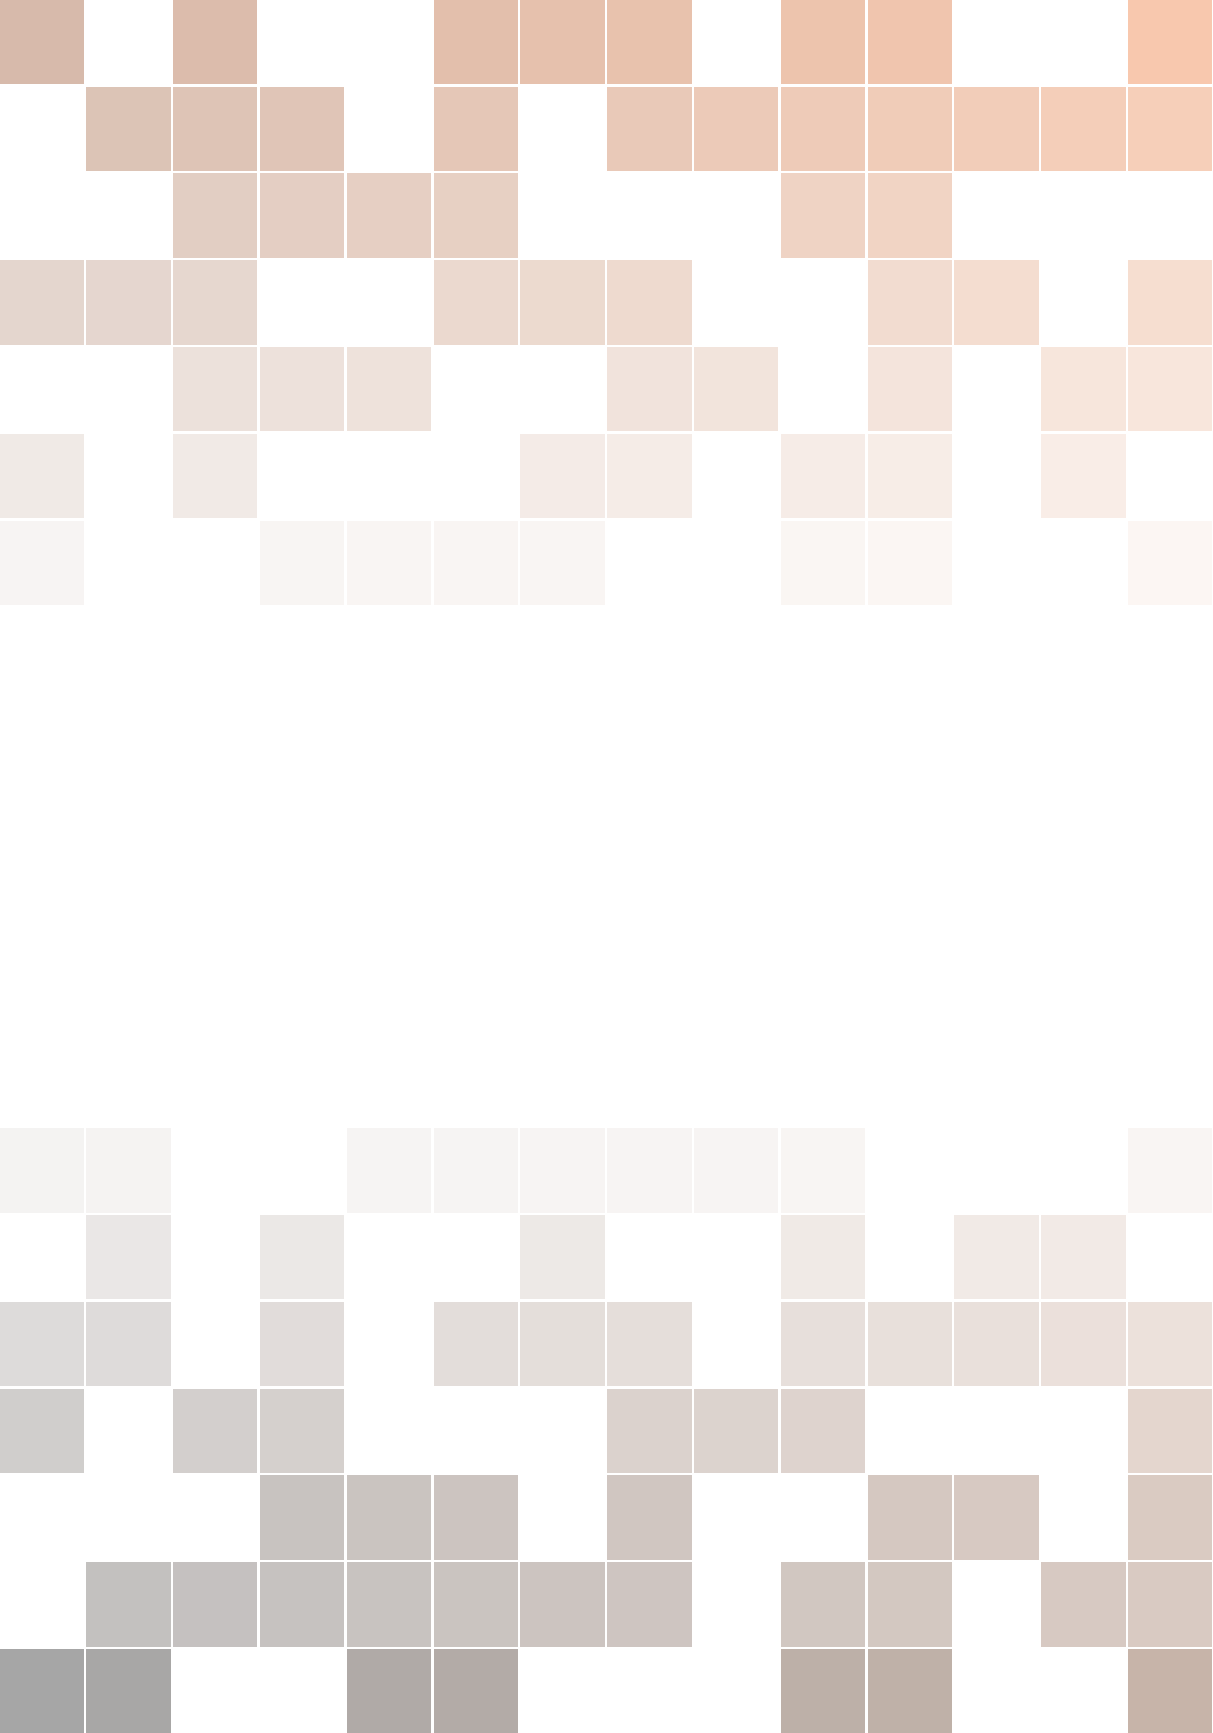
\includegraphics[width=\paperwidth]{images/background}}; % Background image
%\textsl{}
%      \draw[anchor=north] (midpoint) node [fill=ocre!30!white,fill opacity=0.6,text opacity=1,inner sep=1cm]{\Huge\centering\bfseries\sffamily\parbox[c][][t]{\paperwidth}{\centering Coding Interview Essentials\\[15pt] % Book title
%      {\Large - }\\[20pt] % Subtitle
%      {\huge Davide Spataro}}}; % Author name
%    \end{tikzpicture}};
%\end{tikzpicture}
%\vfill
%\endgroup


\includepdf[pages={2},fitpaper=true]{images/book_covers1.pdf}


\usechapterimagefalse % If you don't want to include a chapter image, use this to toggle images off - it can be enabled later with \usechapterimagetrue

%\chapterimage{images/header} % Table of contents heading image

\pagestyle{empty} % No headers

\tableofcontents % Print the table of contents itself

%\lstlistoflistings
%\listoffigures
%\listoftables

%\cleardoublepage % Forces the first chapter to start on an odd page so it's on the right

%pagestyle{fancy} % Print headers again

%!TEX root = ../main.tex
%%%%%%%%%%%%%%%%%%%%%%%%%%%%%%%%%%
% Links:
% http://www.zrzahid.com/the-%E2%80%A9maximum%E2%80%A9-gap%E2%80%A9-problem-%E2%80%A9pigeonhole-%E2%80%A9principle%E2%80%A9/
% https://leetcode.com/problems/maximum-gap/discuss/50667/Solutions-in-C%2B%2B-with-explanation-read-it-and-then-you-get-it
% https://leetcode.com/problems/maximum-gap/discuss/50694/12ms-C%2B%2B-Suggested-Solution
% Difficulty: Companies: 
%%%%%%%%%%%%%%%%%%%%%%%%%%%%%%%%%%


%\begin{figure} \centering 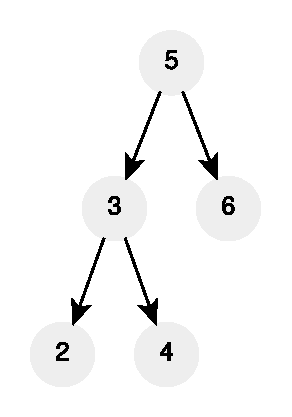
\includegraphics[width=\textwidth]{sources/max_gap/images/example1}
%   \caption[Sample short cpation]{Sample Caption}. \label{fig:max_gap:example1} \end{figure}

\chapter{Find the largest gap}
\label{ch:max_gap}
\section*{Introduction}
The problem discussed in the chapter is another one about sorting. Its statement is quite simple and
the only input given is an unsorted array from which we are asked to calculate a value would be
trivial to find if the input was sorted. Therefore, the real challenge of this problem is to come-up
with a solution that does not require explicit sorting.

Particular attention should be paid to the examples as well as to the problem statement because it
is quite easy to misinterpret the real requirements of the function you asked to write if you dive
right away into coding. The problem asks you to return the largest distance between any element in
the input array provided they appear one next to the other when $I$ is sorted. You might
misinterpret the problem by thinking that you need to return the largest distance between any two
elements of the original input array. This interpretation is wrong, and your intuition should make
you aware of it right away considering that the solution to this problem involves only finding the
minimum and the maximum values of the input array. You can expect any coding interview question to
be harder than that. An imagination effort (or some pen and paper work) is thus necessary to
understand each of the examples provided.

\section{Problem statement}
\begin{exercise}
\label{example:max_gap:exercice1}
Write a function that given a unsorted array of non-negative integers 
$I$ of length $n$ returns the largest gap between two
elements that would appear one next to the other  
if $I$ was sorted. A gap between $x$ and $y$ is defined as the absolute value of the difference
between $x$ and $y$: $|x-y|$.

	%example1
	\begin{example}
		\label{example:max_gap:example1}
		\hfill \\
		Given $I = \{5,3,1,8,9,2,4\}$ the function returns $3$. Sorting $I$ changes it into:
		$sort(I)= \{1,2,3,4,5,8,9\}$, and the largest gap between any two consecutive elements is
		$3$. In this case between $5$ and $8$.		
	\end{example}

	%example2
	\begin{example}
		\label{example:max_gap:example2}
		\hfill \\
		Given $I = \{7, 1, 8, 9,15\}$ the function returns $6$. $sort(I)= \{1,7,8,9,15\}$, and the
		largest gap between any two of its consecutive elements is $6$ e.g. between $1$ and $7$ or
		between $15$ and $9$.	
	\end{example}
	
\end{exercise}

\section{Clarification Questions}

\begin{QandA}
	\item Is the input $I$ modifiable?
	\begin{answered}
		\textit{Yes you can modify $I$.}
	\end{answered}

	\item Is any guarantee or constraint on the value of each element of $I$?
	\begin{answered}
		\textit{You can assume each element of $I$ to fit in a 4 bytes unsigned integer.}
	\end{answered}
	
\end{QandA}

%\section{Discussion} \label{max_gap:sec:discussion}


\section{Trivial Solution}
\label{max_gap:sec:trivial}
As already mentioned in the introduction this problem has an extremely simple solution when we can
afford to get our hands on a sorted version of the input array. In this specific version of the
problem $I$ is not read-only and we are allowed to modify it,therefore, we can sort it directly. If
that is not possible all you have to do is to create a copy of $I$ and sort that instead. 

Given a sorted collection, the largest gap between any two numbers can be find in linear time by
just scanning each pair $p=(I_k, I_{k+1)}$ of subsequent elements and for each of them calculate
their distance $d_k=I_{k-1}-I_k$. Among all calculated distances we just return the largest. Listing
\ref{list:max_gap:bruteforce} shows an implementation of this idea. Notice that:
\begin{itemize}
	\item we do not need to use the absolute value operation as we are operating on a sorted
	collection and therefore, we are guaranteed that $I_{k+1}$ is larger or equal than $I_k$.
	\item the \inline{for} loop stops when $i=|I|-1$ in order to avoid accessing an invalid element
	while executing \inline{I_copy[i+1]}. When $i=|I|-1$ this would lead to accessing the element at index
	$|I|$, which does not exists. In C++ this would cause undefined behaviour, and the most likely
	outcome would be a segmentation fault error.
\end{itemize}
\lstinputlisting[language=c++, caption={Trivial solution to the max gap problem using sorting and linear space.},label=list:max_gap:bruteforce]{sources/max_gap/max_gap_solution1.cpp}



\section{Radix Sort}
\label{max_gap:sec:radix_sort}
The idea we developed in Section \ref{max_gap:sec:trivial} can be improved 
if instead of using a normal comparison-based sorting algorithm  we use 
radix-sort\cite{cit::wiki::radix_sort }instead. 
Radix sort will perform better than a standard $O(nlogn)$ algorithm when there is an upper bound for the values of the 
input array. If we assume that such bound is the largest value a standard 4 bytes \inline{int} can hold then radix sort will 
have a complexity of $O(n)$.

Radix sort works by sorting the input array $d$ times, where $d = \floor{log_{10}k+1}$ and $k$ is the largest number in $I$.
$d$ is just the number of digits of the largest number in the list. For a standard \inline{int} $d=\floor{log_{10}(2147483647) + 1}=10$.
The sorting is obtained by repeatedly sorting the input list from the least to the most significant digit where each of the intermediate 
sorting steps is performed using counting-sort.
For instance given $I = \{329,457,657,839,436,720,355\}$ the first pass of radix sort will sort $I$ based on the value of the least significant digits.
After this first pass we have $I=\{720,355,436,457,657,329,839\}$. Notice how the first digits are sorted. At this point the algorithm proceed by sorting 
$I$ further but this time according to their second digit. The resulting list becomes $I=\{720,329,436,839,355,457,657\}$.
Finally the third pass will sort all the elements according the the most significant digit, resulting in a well
sorted list: $I=\{329,355,436,457,657,720,839\}$. 
Notice that this approach needs to be tweaked in case you want to apply radix sort to negative numbers\footnote{You can treat the sign as a special kind of digit. 
You sort the pile on the units, then the tens, etc. and finally on the sign. 
This does produce a reversed order for the negatives, 
you then simply reverse the contents of that bucket.}.

Listing \ref{list:max_gap:radixsort} shows an implementation of radix-sort and its application to the solution of this chapter's problem.
\lstinputlisting[language=c++, caption={Linear time solution to the max gap problem using radix-sort.},label=list:max_gap:radixsort]{sources/max_gap/max_gap_solution2.cpp}
Notice how the main driver function \inline{max_gap_radix_sort} is basically the same as \inline{max_gap_bruteforce} from Listing \ref{list:max_gap:bruteforce} except for the sorting procedure used.

\section{Buckets and the pigeonhole principle}
\label{max_gap:sec:buckets}
All the solutions we have presented so far rely on sorting. In this section we are going to discuss an approach
that rely on  the pigeonhole principle\footnote{\url{https://en.wikipedia.org/wiki/Pigeonhole_principle}} and bucketing.
The general idea is that we could split the entire array into several buckets and then find the largest gap by only comparing
one element of a given bucket to one element of the subsequent bucket. 

You can think of $I$ as an array of buckets each containing a single element. $|I|$ is made of $b$ buckets and the total amount of element in $I$ is $n=b$.
Imagine for a moment that you would reduce the number of buckets from $b$ to some integer $k < b$.
For the pigeonhole principle then, one or more of the buckets in $I$ have to contain  strictly more than one element.

Let's now focus for a moment of the gaps of an ideal collection where each of the elements has a given distance $t$ from its successor in the list. 
If such a collection ic composed of  $n$ elements, then there is a total of $n-1$ gaps, each of size $t$.
$t$ can be easily calculate if the maximum and minimum values are known: in-fact $t=\frac{max-min}{n-1}$. 
If $I$ was like this ideal collection then the problem would be easily solved by using the formula above. 
$I$ is different to this ideal collection because elements do not have uniform gaps between each other. 
In this situation then we can argue that the maximum gap between any pair of subsequent 
elements of $I$ is always larger than $t$.
We can show this by trying reduce the gap between two subsequent elements $I_{i}$ and $I_{i+1}$, of an ideal collection with uniform gaps.
We can do that by moving $I_{i+1}$ closer to $I_{i}$. When this happens the gap $(I_{i+1}-I_{i})$ becomes smaller than $t$. But what happens to the gap between $I_{i+1}$ and $I_{i+2}$?
It actually becomes larger than $t$. In our effort to make the largest gap among two subsequent elements smaller, we obtained the opposite result: we made it larger.
This shows that the maximum attainable gap can in a  collection with uniform gaps can only increase. 

We are going to apply the two ideas above to solve this problem in the following way. We will distribute all the element of $I$
into $n-1$ buckets. The first bucket would contains all the elements of $I$ which have in the following range: $[min, min + t)$.
Similarly the second buckets would contain all the elements in the following range: $[min + t, min + 2t)$. 
In general the $i^{th}$ bucket  would contain all the elements of $I$ in the following range: $[min + (i-1)t, min +it)$ (where $ 1 \leq i$).
You can refer to Figure \ref{fig:max_gap:bucketing_example2} for an example of how such a division into buckets would work for the input array in Example \ref{example:max_gap:example2}.
This allows us to skip comparing all the element within a bucket because we know for sure they will have a distance that is lower of equal than $t$ and we can therefore only concentrate on comparing elements 
of subsequent buckets.
In particular we should compare the maximum value of the $i^{th}$ bucket with the minimum value of the $(i+1)^{th}$ bucket. Why? Because they would appear one next to the other if $I$ was sorted.
Because the number of buckets is always lower of equal than the number of elements in the collection, this approach has a linear complexity as it does require to compare at most twice the number of input elements in $I$.


\begin{figure}
	 \centering
	 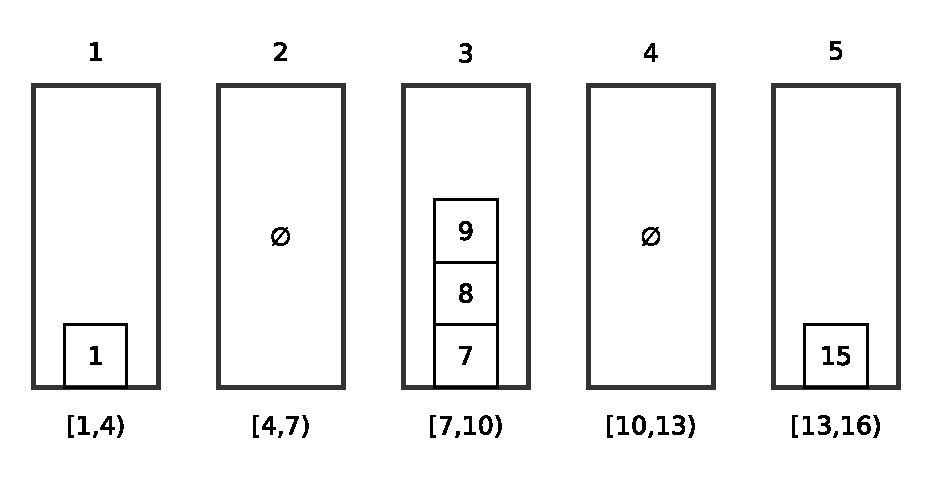
\includegraphics[width=\textwidth]{sources/max_gap/images/bucketing_example1}
     \caption{Division of the elements of the Example \ref{example:max_gap:example2} into buckets.}.
	\label{fig:max_gap:bucketing_example2}
\end{figure}



%%%%%%%%%%%%%%%%%%%%%%%%%%%%%%%%%%%%%%%%%%%%
%               Appendices
%%%%%%%%%%%%%%%%%%%%%%%%%%%%%%%%%%%%%%%%%%%%

\chapter{Appendices}
%% @Author: Davide Spataro
% @Date:   2020-10-25 
% @Last Modified by:   Davide Spataro
% https://www.topcoder.com/community/competitive-programming/tutorials/dynamic-programming-from-novice-to-advanced/
% file:///home/knotman/Downloads/DYNAMIC_PROGRAMMING_-_ITS_PRINCIPLES_APPLICATIONS_.pdf
% http://smo.sogang.ac.kr/doc/bellman.pdf 
\section*{Dynamic Programming}
\label{sect:appendix:DP}

Dynamic programming (DP) is a popular technique for solving a certain class of
optimization problems efficiently and is accredited to the American Scientist
Richard Bellman\cite{bellman1954}. He conied the term DP in the context of
solving problems involving a serie of best decision one after the other. 
The word \textit{programming} can be a bit deceiving for
computer scientist of programmers in general but it has really little to do with
computer programming and it is infact intended as a set of rules to 
follow to solve a certain problem and it is refeered specifically to the
solution to find an optimal military schedule for logistics (and has more or
less the same meaning as linear programming or linear optimization).  These rules can of course be coded and
executed by a computer but can be easily followed on paper for instance. 
Dynamic programming is better thought as an optimization approach rather than an
method or framework where a complex optimization problem is transformed into a sequence of
smaller (and simpler) problems. The very essence of DP is its multi-stage
optimization procedure. DP does not provide directly with the
instruction on how to solve a particular problem, but instead provides a general
framework that requires creativity and non trivial effort/insights so that a
problem formulation can be adapted and casted within the DP framework bounds.
This is possibly the reason why DP is considered a rather hard topic and it is
particularly feared during interviews. 

This chapter is not intended to be a full treatement of DP, and we will
introduce and describe it to the level that is necessary to understand and
better tackle DP interview problems. For a more comprenshive material on DP
please refer to \cite{bellman1954, cormen2009}.

The gist of the DP approach is that we aim at breaking down a problem into
simpler sub-problems recursively. If it is possible to do so, then the problem
at hand is said to have the \textbf{optimal substructure} property i.e. it can
be solved by using optimal solution to subproblems. But having the optimal
substructure property alone is not enough to prefer a DP approach to another
when trying to solve the same problem. This is because DP really shines when a
problem also exposes the \textbf{overlapping subproblems} property i.e. when the
subproblems are reused several times. A classic example if the
Fibonacci Sequence. In order to calculate $F(n)$ we need to solve two subproblems:
$F(n-1)$ and $F(n-2)$ and adding them up. But for solving $F(n-1)$ we need to
solve $F(n-2)$ \textbf{again}. The value for the subproblem $F(n-2)$ is thus
reused and this makes the Fibonacci problem exposed the optimal substructure
property. 
Dynamic programming takes care of this fact by making sure of solving each
subproblem only once. Usually this can be achieved into two ways:
\begin{description}
    \item [Top-down] This is usually the easiest of the two, by being a direct
    derivation from the recursive formulation of the problem. If the problem can
    be formulated recursively in terms of solution then solution to subproblems
    can be \textit{memoized}\footnote{From the latin word \textit{memorandum}
    which means to be remembered. It is basically a way of remembering the
    result of a function for a certain set of inputs call by storing it in a
    cache.} in a cache. 
    When a subproblem is reused then the
    (potentially expensive) recursive call is avoided and the cached result is
    returned instead. 
    \item [Bottom-up] We can try to reformulate the problem by twisting and
    massaging  the  recursive formulation so that the subproblems are solved
    first (thus effectively removing the recursion) and build the solution to
    the bigger problem from the bottom. This is usually done by working in a
    sort of tabular form where entries of the table for larger problems are
    filled by using  entries for solution to smaller problems that we have
    already solved. For instance, when solving the problem of finding the
    $10^{th}$ Fibonacci number $F(10)$, we can start from the known values for
    $F(0)$ and $F(1)$ and working our way up to $F(2)$  by using $F(1)$ and
    $F(2)$. Once F(2) is ready we can move up to F(3), and so on when we have
    the values for $F(8)$ and $F(9)$ we proceed with calculating $F(10)$.
\end{description}

DP has found application in many field of science such as Control theory,
Bioinformatics AI and operations research. There are a number of problems in
computer science that can be solved by using DP such as the 
\begin{itemize}
    \item Longest Common (or increasing) Subsequence
    \item Weighted Interval Scheduling
    \item Chain Matrix Multiplication
    \item Subset sub
    \item String edit distance
    \item Coin change
    \item 0/1 knapsack problem
    \item Graph shortest path
\end{itemize}

In the next section we will shortly review a number of DP problem focusing on
the key ideas that allow a problem to be approached and solved  using DP.

\subsection*{Fibonacci Sequence}
Computing the $n^{th}$ number of the Fibonacci sequence is probably one of the
most common introductionary example of DP. The Fibonacci sequence recursive
formulation is ready to be solved using a top-down DP approach. Listing
\ref{list:app:dp:canonical} shows a C++ function that calculated the $n^{th}$ Fibonacci
number.
\lstinputlisting[language=c++, caption={Canonical recursive C++ implementation of a function returning the $n^{th}$ Fibonacci number.},label=list:app:dp:canonical]{/home/dspataro/git/algorithm_articles/sources/appendices/fibonacci_canonical.cpp}
Notice that for instance when $F(6)$ a call tree is produced where the same call
is repeated more than once as shown in the list below. $F(2)$ has been
calculated $5$ times!
\begin{itemize}
    \item $F(6) = F(5)+F(4)$
    \item $F(6) = (F(4)+F(3)) + (F(3)+F(2))$
    \item $F(6) = ((F(3)+F(2))+(F(2)+F(1))) + ((F(2)+F(1))+(F(1)+F(0)))$
    \item $F(6) = (((F(2)+F(1))+(F(1)+F(0)))+((F(1)+F(0))+F(1))) + (((F(1)+F(0))+F(1))+(F(1)+F(0)))$
    \item $F(6) = ((((F(1)+F(0))+F(1))+(F(1)+F(0)))+((F(1)+F(0))+F(1))) + (((F(1)+F(0))+F(1))+(F(1)+F(0)))$
\end{itemize}

Listing \ref{list:app:dp:fib} can be improved dramatically if we memoize the function calls
that have been already calculated. This way no duplicate work is done. W.r.t the
previous example, from the second time the value of $F(2)$ is needed, no
additional work is done, as the value in the cache is returned.
\lstinputlisting[language=c++, caption={Canonical recursive top-down Dynamic Programming C++ implementation of a function returning the $n^{th}$ Fibonacci number.},label=list:app:dp:fib]{/home/dspataro/git/algorithm_articles/sources/appendices/fibonacci_dp_top_down.cpp}

%\section{Prefix sum}
\label{sect:appendix:prefix_sum}
In computer science, the prefix sum, cumulative sum, inclusive scan, or simply scan of a sequence of numbers x0, x1, x2, ... is a second sequence of numbers y0, y1, y2, ..., the sums of prefixes (running totals) of the input sequence:
%% @Author: Davide Spataro
% @Date:   2020-03-30 17:18:14
% @Last Modified by:   Davide Spataro
% @Last Modified time: 2020-03-30 17:28:08
\section{Binary Search}
\label{sect:appendix:binary_search}
\lipsum{1}
%%%%%%%%%%%%%%%%%%%%%%%%%%%%%%%%%%%%%%%%%%%%
%               BIBLIOGRAPHY
%%%%%%%%%%%%%%%%%%%%%%%%%%%%%%%%%%%%%%%%%%%%

%
%from documentation
%\newacronym[⟨key-val list⟩]{⟨label ⟩}{⟨abbrv ⟩}{⟨long⟩}
%above is short version of this
% \newglossaryentry{⟨label ⟩}{type=\acronymtype,
% name={⟨abbrv ⟩},
% description={⟨long⟩},
% text={⟨abbrv ⟩},
% first={⟨long⟩ (⟨abbrv ⟩)},
% plural={⟨abbrv ⟩\glspluralsuffix},
% firstplural={⟨long⟩\glspluralsuffix\space (⟨abbrv ⟩\glspluralsuffix)},
% ⟨key-val list⟩}

\newacronym{cd}{CD}{compact disk}
\newacronym{utc}{UTC}{Coordinated Universal Time}
%\newacronym{adt}{ADT}{Atlantic Daylight Time}
%\newacronym{est}{EST}{Eastern Standard Time}
 
% Use the acronyms
\gls{utc} is 3 hours behind \gls{adt} and 10 hours ahead of \gls{est}.



%\addcontentsline{toc}{chapter}{\textcolor{ocre}{Glossary}}
%\printglossaries


%Print the glossary

\addcontentsline{toc}{chapter}{\textcolor{ocre}{Bibliography}}
%\chapter*{Bibliography}
%Print the glossary
\printbibliography	
	
%%%%%%%%%%%%%%%%%%%%%%%%%%%%%%%%%%%%%%%%%%%%
%               INDEX
%%%%%%%%%%%%%%%%%%%%%%%%%%%%%%%%%%%%%%%%%%%%	
	\cleardoublepage
	\phantomsection
	\setlength{\columnsep}{0.75cm}
	\addcontentsline{toc}{chapter}{\textcolor{ocre}{Index}}
	\printindex


	%\backmatter

\end{document}
